\chapter{Investigation of reflection at media interface}
Here we investigate how much energy is reflected and how much is transmitted at the media interface. We had considered lossless medium in d previous lectures for which $ \sigma $=0, but with different permeability and permittivity.

We already established that knowing $E_{1}$ it can also be found from $\frac{E}{H} = \eta$ relation.
\begin{figure}[h]
\centering
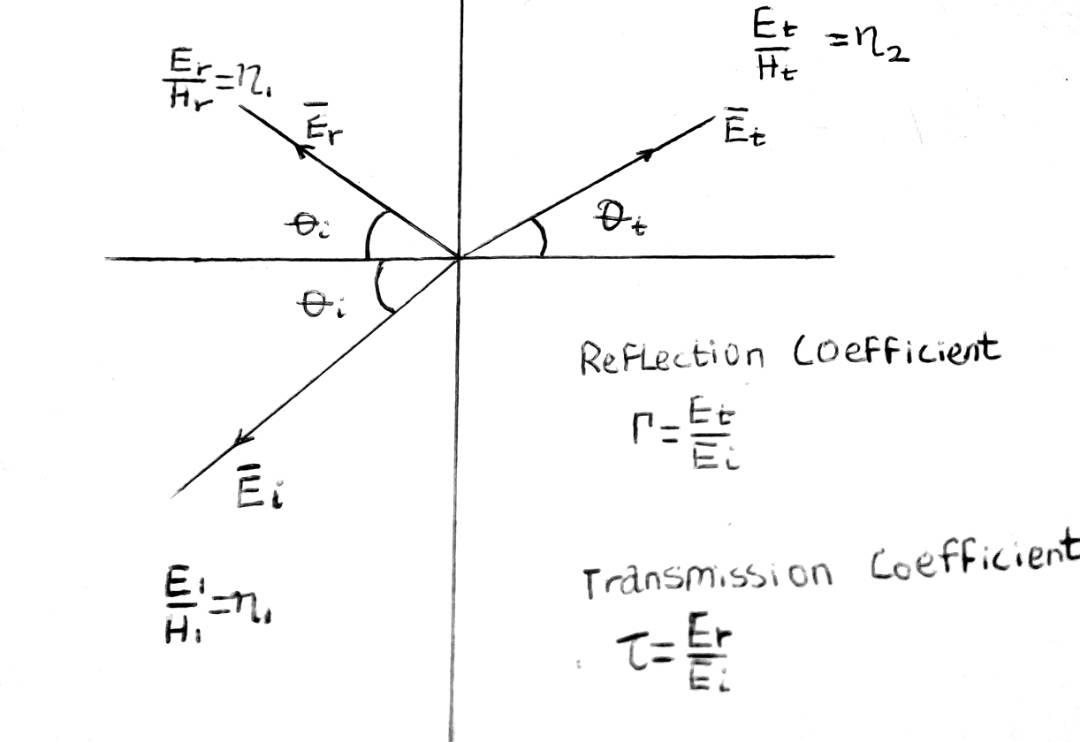
\includegraphics[width=1\linewidth]{./graphics/11}
\caption{}
\label{fg:11}
\end{figure}

Again E at an arbitrary angle to the plane of incidence is resolved to parallel polarized and perpendicular polarized i.e along the plane of incidence and normal to the plane of incident respectively.

so write down the electric and magnetic field for the two media and then apply boundary condition at the interface and by some algebra we get $\frac{E_{r}}{E_{i}}$ and $\frac{E_{t}}{E_{i}}$ for reflection coefficient and transmission coefficient respectively.

So we find out the $\Gamma$ and $\tau$ for each of the two cases of parallel and perpendicular polarization for each of the two cases.

\section{Perpendicular polarization} 
From the diagram below the wave is incident at an angle $\theta_{i}$ to the normal. The wave vector lies on the paper or the plane of incidence. For perpendicular polarization either the electric field is coming out of the paper in the positive y direction or going into the paper in the negative y direction.
\begin{figure}[h]
\centering
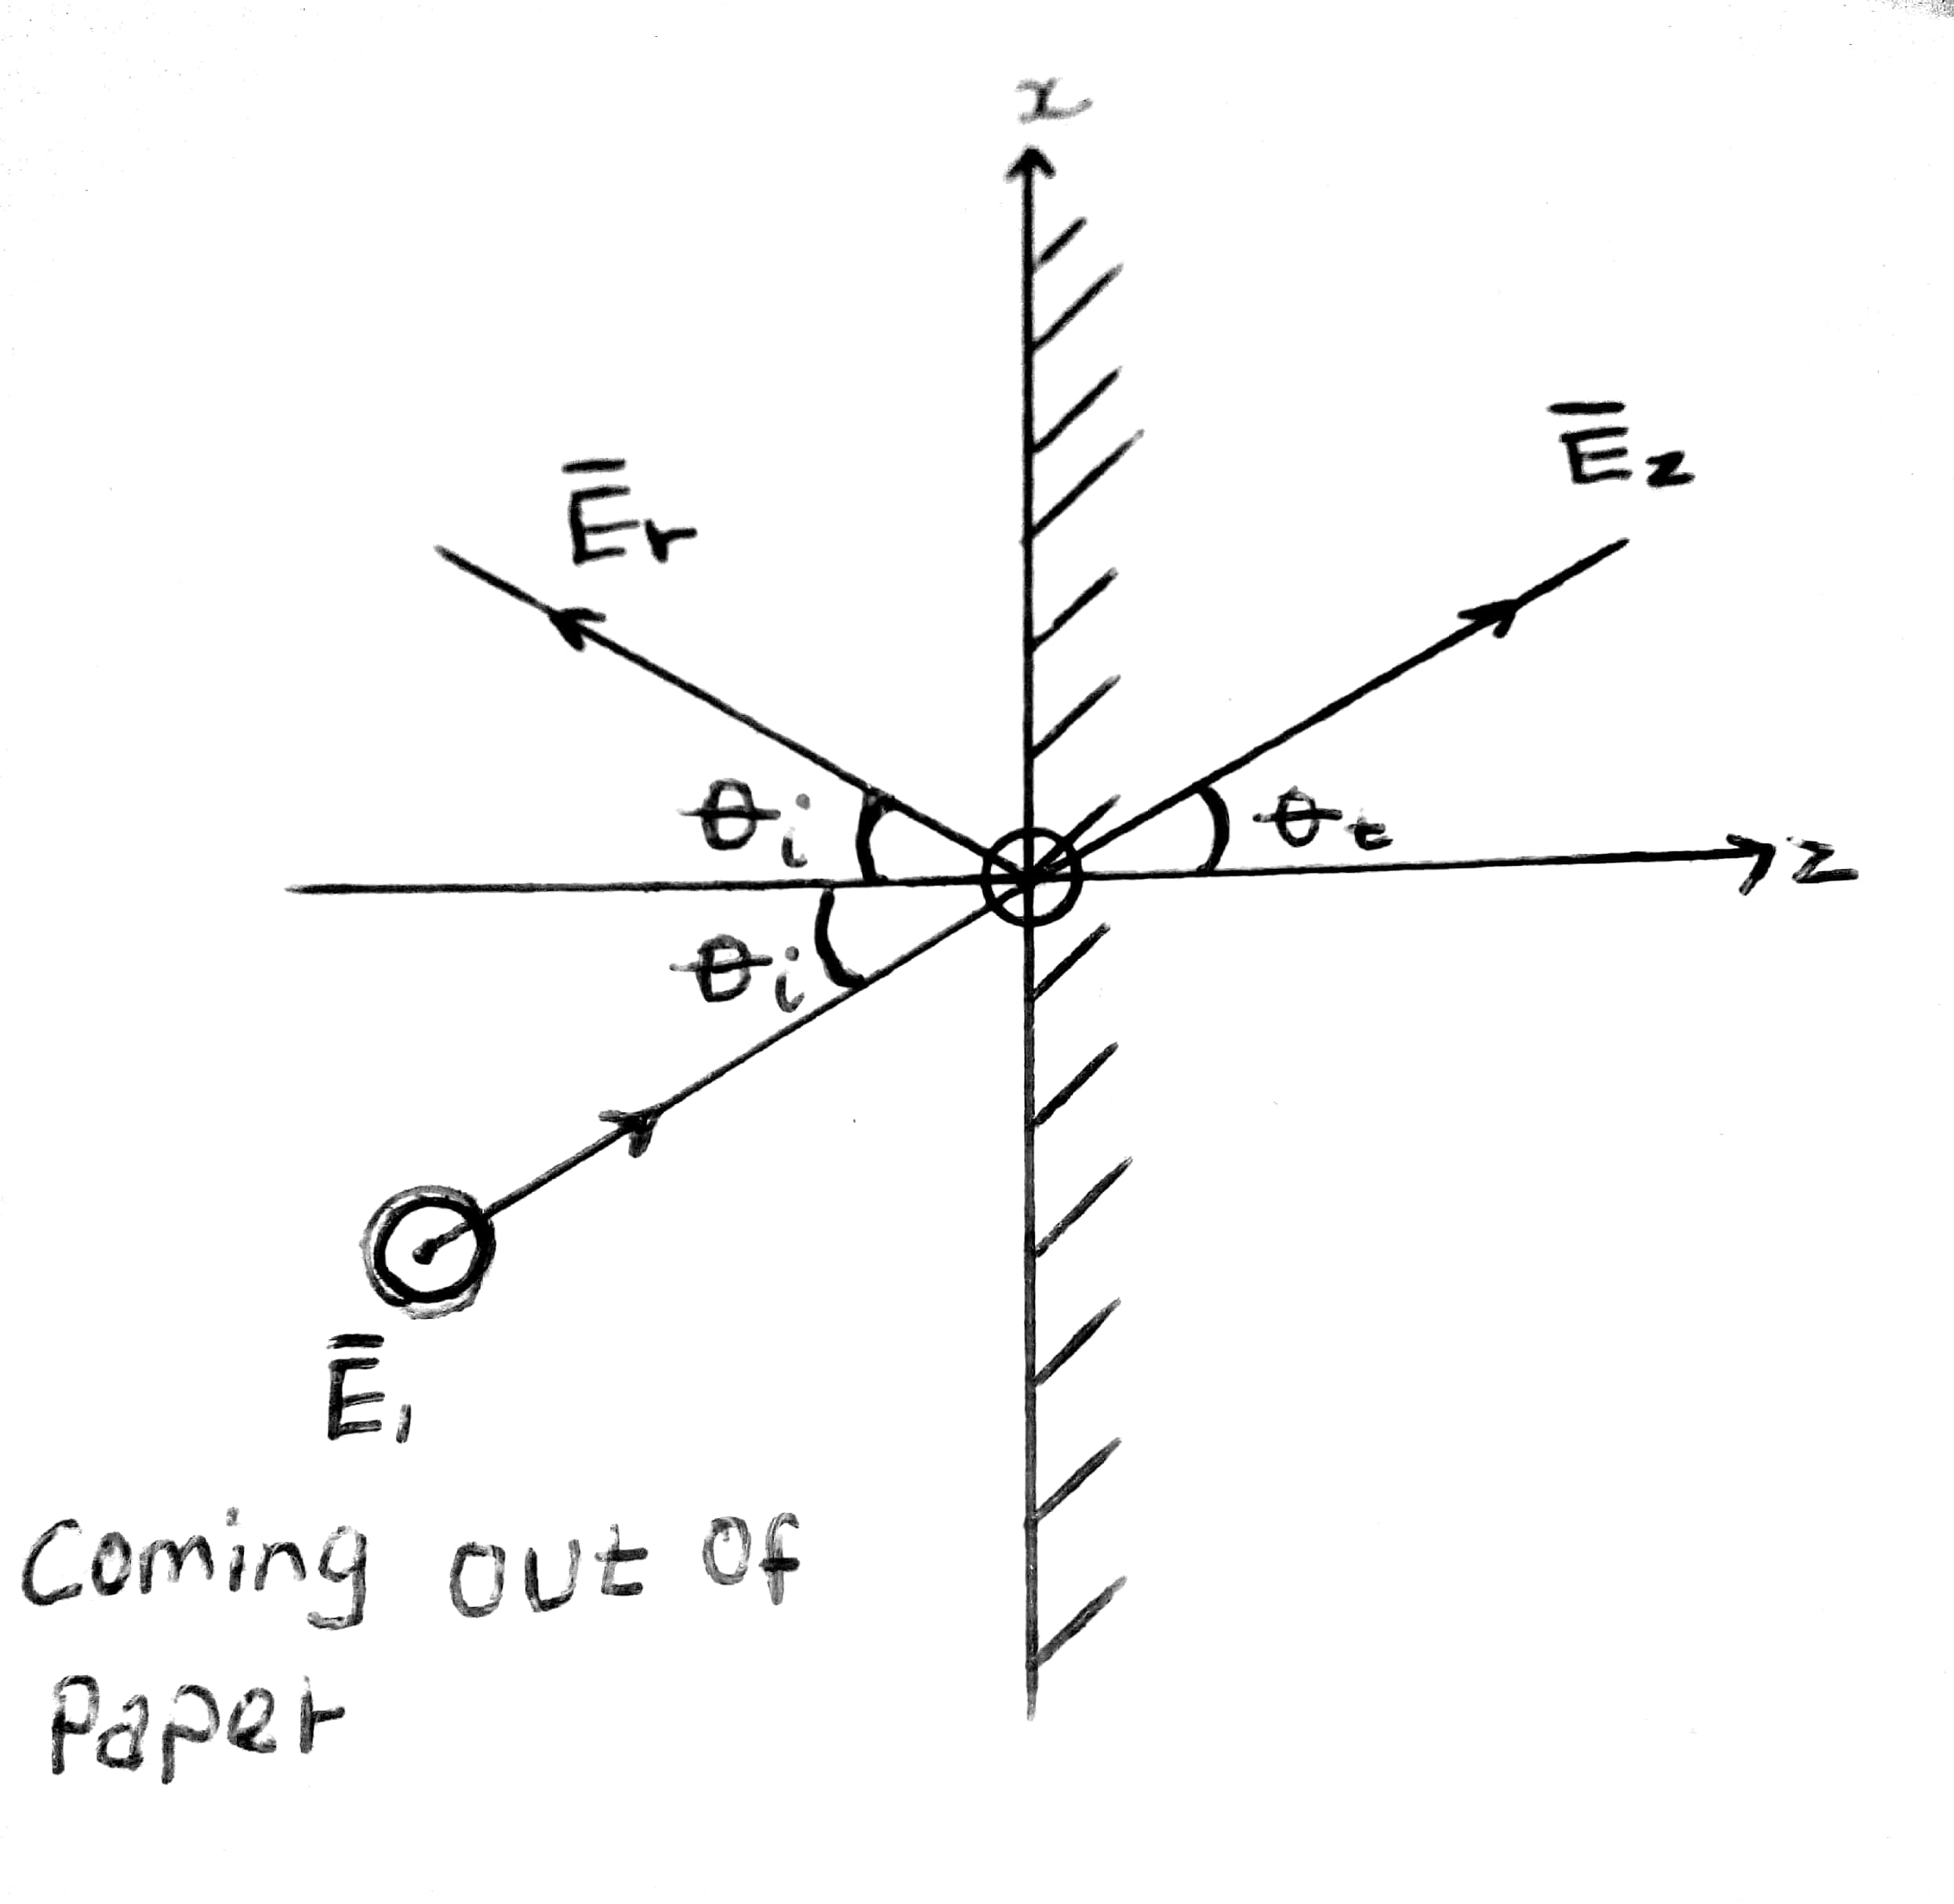
\includegraphics[width=1\linewidth]{./graphics/12}
\caption{}
\label{fig:12}
\end{figure}

We can argue that to satisfy the boundary condition, at the interface, the tangential component of an electric field across the boundary should be continuous. If $\bar{E}_{i}$ is y oriented both  $\bar{E}_{r}$ and  $\bar{E}_{t}$ must be y oriented.
\begin{figure}[h]
\centering
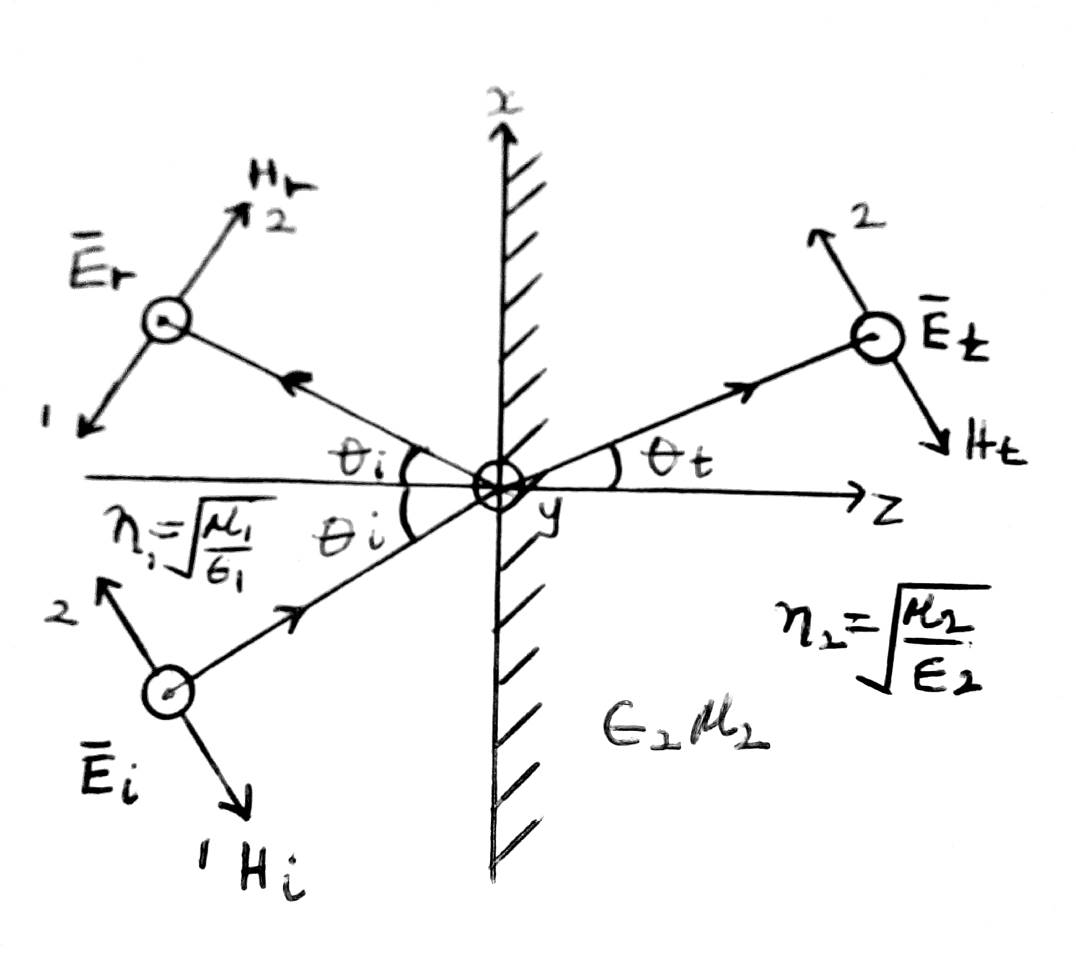
\includegraphics[scale=0.2]{./graphics/13}
\caption{}
\label{fig:13}
\end{figure}

$\bar{E}_{r}$ and  $\bar{E}_{t}$ may not necessarily be in the positive y direction but it is in the y direction. let us just say it is in the positive y direction so  $\bar{E}_{i}$,  $\bar{E}_{t}$ and  $\bar{E}_{r}$ are all assumed to be coming out of the plane of the paper. We have to write down the corresponding magnetic field for which we use the pointing Vector argument. We must choose the direction of magnetic field H such that the pointing vector will be in the direction of the wave propagation or wave vector. Since E for all 3 electric fields is perpendicular to the plane of the paper, the H field vector for all 3 must lie in the place of the paper or plane of the incident. They can go in directions 1 or 2 shown in the diagram as far as H is on the plane of the paper. 1 or 2 will be decided by pointing vector of  $\bar{E} \times \bar{H}$ giving the wave direction since we are dealing with transverse electromagnetic waves $\frac{E}{H} = \eta$. So that $\frac{E_{i}}{H_{i}} = \eta_{1}$, $\frac{E_{r}}{H_{r}} = \eta_{1}$, $\frac{E_{t}}{H_{t}} = \eta_{2}$.

Again we decompose the magnetic field into components along x and z. E is already perpendicular to the plane of the paper. We bring it out clearly in figure~\ref{fig:14}.
\begin{figure}[h]
\centering
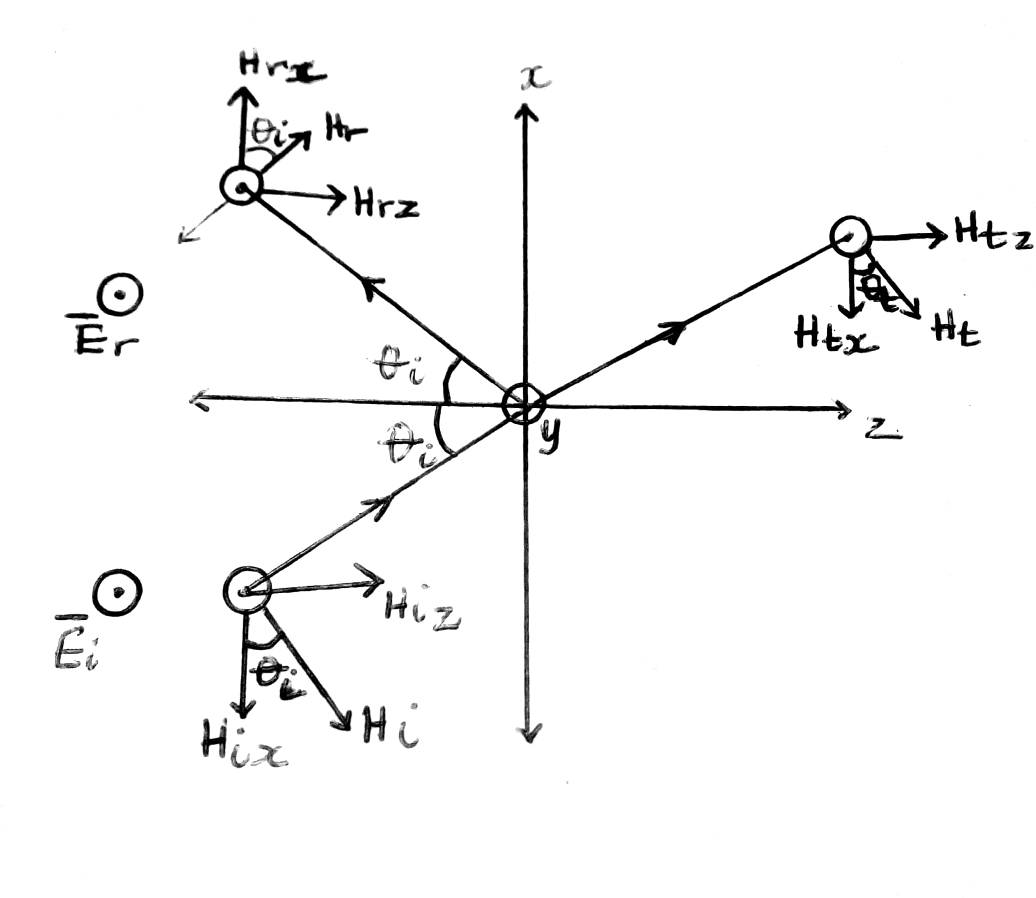
\includegraphics[width=1\linewidth]{./graphics/14}
\caption{}
\label{fig:14}
\end{figure}

From figure~\ref{fig:14} the following can be evaluated
\begin{align*}
\bar{E_{i}} = E_{1} \varrho^{-j\beta_{1}} (x sin\theta_{i} + z cos\theta_{i}) \hat{y}\\
\bar{E_{r}} = E_{r}  \varrho^{-j\beta_{1}} (x sin\theta_{i} - z cos\theta_{i}) \hat{y}\\
\bar{E_{t}} = E_{t} \varrho^{-j\beta_{2}} (x sin\theta_{t} + z cos\theta_{t}) \hat{y}
\end{align*}
All electric field has been written out explicitly 

If they have to satisfy the boundary condition and since all 3 fields are tangential to the boundary, at the dielectric boundary, $z=0$. The sum of $E_i$ and $E_r$ should be equal to $E_{t}$. From the boundary condition, the tangential component of E should be continuous at $z=0$ I.e the inter-phase.
\begin{align*}
E_{i} \varrho^{-j \beta_{i} x sin\theta_{i}} + E_{r} \varrho^{-j \beta_{1} x sin\theta_{1}} = E_{t} \varrho^{-j \beta_{2} x sin\theta_{2}}
\end{align*}
We recall from snells law that $\beta_{i} x sin\theta_{i} = \beta_{1} x sin\theta_{1} = \beta_{2} x sin\theta_{2}$. Hence the phase function is the same for all the 3 waves, hence the phase term is common.

This implies that $ E_{i} + E_{r} = E_{t}$. This relationship is true whether for normal or tangential components since this phase gradient is the same. So the component we take for electric or magnetic field is immaterial, as this phase function remains the same.do whatever boundary condition is satisfied, this phase function is always the same so that the boundary condition can be applied only to the amplitude term. 
\begin{equation}
E_{i} + E_{r} = E_{t}
\end{equation}
Since we are talking about dielectric media, there are no surface currents, we can also use the continuity of the tangential component of the magnetic field. The tangential component continuity can not be assumed if there is the possibility of surface current. As we have seen surface current is for conductors. So with a dielectric boundary like this no surface current, the continuity of the tangential component of the magnetic field can be applied. So that 
\begin{center}
$H_{i} cos\theta_{i} - H_{r} cos\theta_{i} = H_{t} cos\theta_{t}$
\end{center}
\begin{equation}
\frac{E_{i}}{\eta_{1}} cos\theta_{i} - \frac{E_{r}}{\eta_{1}} cos\theta_{i} = \frac{E_{t}}{\eta_{2}} cos\theta_{t}
\end{equation}
We are interested in finding out two components $\Gamma = \frac{E_{r}}{E_{i}}$ and $ \tau = \frac{E_{t}}{\eta_{i}}$, we use these two equations to find out these quantities:
\begin{enumerate}[(i)]
\item REFLECTION COEFFICIENT FOR PERPENDICULAR POLARIZATION
$$\Gamma_{\bot} = \frac{\eta_{2} cos\theta_{i} - \eta_{1} cos\theta_{t}}{\eta_{2} cos\theta_{i} + \eta_{1} cos\theta_{t}}$$
\item TRANSMISSION COEFFICIENT
$$\tau_{T} = \frac{2 \eta_{2} cos\theta_{i}}{\eta_{2} cos\theta_{i} + \eta_{1} cos\theta_{2}}$$
\end{enumerate}
Dividing equation 2.1 by $H_{r}$ , we have
\begin{equation}
\centering
\frac{E_{i}}{H_{r}} + \frac{E_{r}}{H_{r}} = \frac{E_{t}}{H_{r}}
\end{equation}
or
$$1 + \Gamma = \tau$$
\begin{equation*}
\frac{1}{\eta_{1}}cos\theta_{i} - \frac{\Gamma}{\eta_{1}}cos\theta_{i} = \frac{\tau}{\eta_{2}}cos\theta_{t}
\end{equation*}
but $1 + \Gamma = \tau$
\begin{dmath*}
\frac{1}{\eta_{1}}cos\theta_{i} - \frac{\Gamma}{\eta_{1}}cos\theta_{i} = \frac{1+\Gamma}{\eta_{2}}cos\theta_{t} = \frac{1}{\eta_{2}}cos\theta_{t} + \frac{\Gamma}{\eta_{2}}cos\theta_{t}
= \Gamma( \frac{1}{\eta_{2}}cos\theta_{t} + \frac{1}{\eta_{1}}cos\theta_{i})
\end{dmath*}
$$\eta_{2}cos\theta_{i} - \eta_{1}cos\theta_{t} = \Gamma(\eta_{1}cos\theta_{t} + \eta_{2}cos\theta_{i})$$
So
$$\Gamma = \frac{\eta_{2}cos\theta_{i} - \eta_{1}cos\theta_{t}}{\eta_{2}cos\theta_{i} + \eta_{1}cos\theta_{t}}$$
and
\begin{dmath*}
\tau = 1 + \Gamma = 1 + \frac{\eta_{2}\cos\theta_{i} - \eta_{1}\cos\theta_{t}}{\eta_{2}\cos\theta_{i} + \eta_{1}\cos\theta_{t}}
= \frac{\eta_{2}\cos\theta_{i} + \eta_{1}cos\theta_{t} + \eta_{2}cos\theta_{i} - \eta_{1}cos\theta_{t}}{\eta_{2}\cos\theta_{i} + \eta_{1}\cos\theta_{t}} = \frac{2 \eta_{2}\cos\theta_{i}}{\eta_{2}\cos\theta_{i} + \eta_{1}\cos\theta_{t}}
\end{dmath*}
hence for the perpendicular polarization
\begin{dmath}
\Gamma_{\perp} = \frac{\eta_{2}cos\theta_{i} - \eta_{1}cos\theta_{t}}{\eta_{2}cos\theta_{i} + \eta_{1}cos\theta_{t}}
\end{dmath}
\begin{dmath}
\tau_{\perp} = \frac{2 \eta_{2}cos\theta_{i}}{\eta_{2}cos\theta_{i} + \eta_{1}cos\theta_{t}}
\end{dmath}
So just after the boundaries, if we find out what are the electric fields, the reflection coefficient gives us what will be the electric field before the boundary and the transmission coefficient gives us what will be the electric field just after the boundary.

Once $E_{r}$ and $E_{t}$ are obtained, then we have the phase function. We can find out the wave at any location at any point in space in medium 1 and in medium 2. In medium  1, we have a superposition of the wave $E_{r}$ and $E_{i}$.

In medium 2 we have only $E_{t}$. Two things are observed for transmission band and reflection  coefficient
\begin{enumerate}[(i)]
\item the reflection coefficient is always  less than 1 or $|\Gamma_{\bot}| \leq 1$ but $\tau_{\bot}$ could be less than 1 or greater than 1. The pointing vector is proportional  to $|\bar{E}|^{2}$. So if $|\Gamma|< 1$, that means the pointing vector magnitude for the reflected wave is always less than  1. So the power density of the reflected wave is always going to be less than that of the incident wave.  $\tau_{\bot} > 1$ means the electric field in medium 2 will be larger than that of the incident electric field. This does not mean that the pointing vector in 2(representing power density) is more than that of medium 1.

\item Although the electric field is larger in medium 2, the intrinsic impedance $\eta=\sqrt{\frac{\mu}{\epsilon}}$.

it is less in medium 2 since $\frac{E}{\eta} =H$. The law of conservation of energy must hold. The power density incident must be equal to the power density transmitted plus the power density reflected.

Though the electric field in medium 2 will be larger, their Poynting vector will be less compared to that for the incident wave.

When a wave is reflected from the boundary, this may be a phase reversal for the wave or there may be no phase reversal for the wave. The incident wave and transmitted wave are always in phase at $\tau$ and are always positive, $\Gamma$ can be positive or negative.
\end{enumerate}
Hence $E_{i}$ and $E_{r}$ can be in phase ($\Gamma_{\perp}$ positive) or out of phase i.e $\Gamma_{\perp}$ is negative. This means that $E_{i}$ and $E_{t}$ will always be coming out of the paper, where the reflected wave $E_{r}$ and $E_{i}$ can be coming out of the paper(when $\Gamma_{\perp}$ is positive).

$E_{r}$ can be going into the paper(while $E_{i}$ is coming out) for $\Gamma_{\perp}$ negative. This is the important conclusion that we can draw for this perpendicularly polarized wave

\section{Parallel polarization}
With $H$l coming out of the paper E lies on the paper or the plane of incidence. The phase function is the same and there is continuity of the tangential component of the magnetic field.
We get $H_{i} + H_{r} = H_{t}$ or
\begin{figure}[h]
\centering
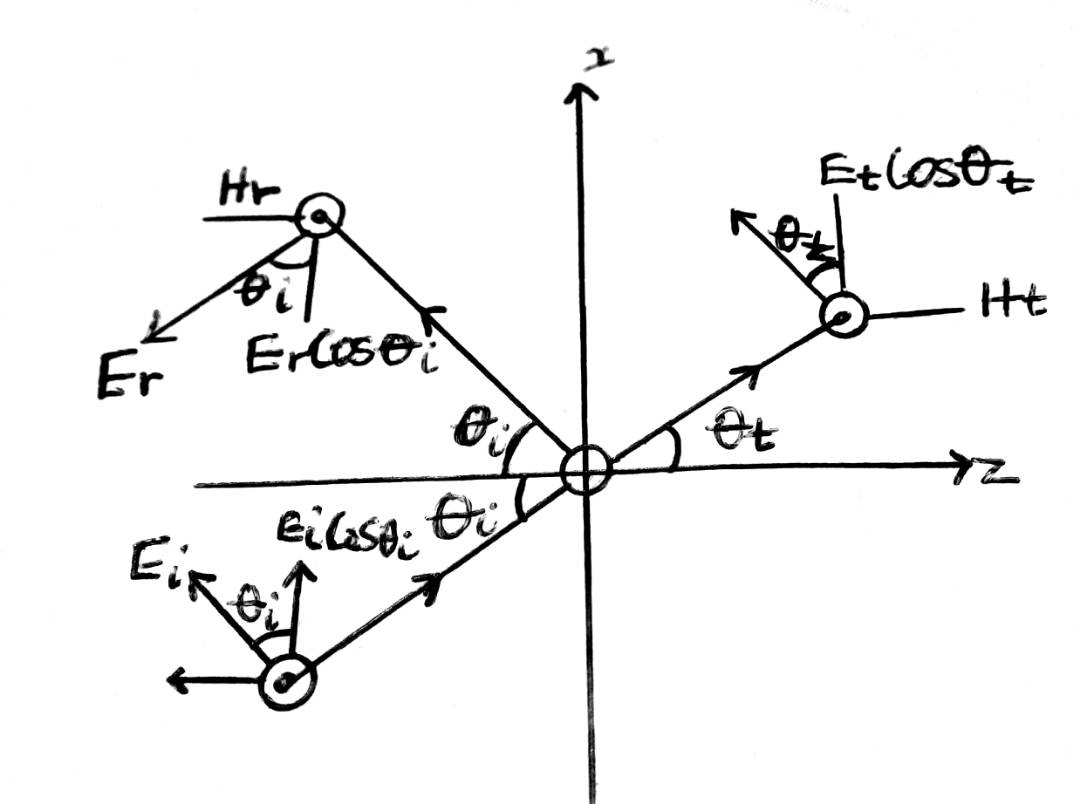
\includegraphics[width=1\linewidth]{./graphics/15}
\caption{}
\label{fig:15}
\end{figure}

\begin{equation}
\frac{E_{i}}{\eta_{1}} + \frac{E_{r}}{\eta_{1}} = \frac{E_{t}}{\eta_{2}}
\end{equation}
\begin{equation}
E_{i} cos\theta_{i} - E_{r} cos\theta_{i} = E_{t} cos\theta_{t}
\end{equation}
divide equation 2.6 by $E_{i}$ we have
\begin{equation}
\frac{1}{\eta_{1}} + \frac{\Gamma}{\eta_{1}} = \frac{\tau}{\eta_{2}}
\end{equation}
divide equation 2.7 by $E_{i}$ to have
\begin{equation}
cos\theta_{i} - \Gamma cos\theta_{i} = \tau cos\theta_{t}
\end{equation}
\begin{equation*}
\tau = \frac{1}{cos\theta_{t}} (cos\theta_{i} + \Gamma cos\theta_{i})
\end{equation*}
substituting in equation 2.8 to have
\begin{align*}
\frac{1}{\eta_{1}} + \frac{\Gamma}{\eta_{1}} &= \frac{1}{\eta_{2}} \frac{1}{\cos\theta_{t}} (\cos\theta_{i} + \Gamma \cos\theta_{i})\\
\frac{1}{\eta_{2}} - \frac{\cos\theta_{i}}{\eta_{2} \cos\theta_{t}} &= - \frac{\Gamma}{\eta_{1}} - \frac{\Gamma cos\theta_{i}}{\eta_{2} \cos\theta_{t}}\\
\Gamma \left(\frac{1}{\eta_{1}} + \frac{\cos\theta_{i}}{\eta_{2} cos\theta_{t}}\right) &= \frac{cos\theta_{i}}{\eta_{2} \cos\theta_{t}} - \frac{1}{\eta_{1}}\\
\Gamma \left(\frac{\eta_{2} \cos\theta_{t} + \eta_{i} \cos\theta_{i}}{\eta_{1} \eta_{2} \cos\theta_{t}}\right) &= \frac{\eta_{1} cos\theta_{i} + \eta_{2} \cos\theta_{t}}{\eta_{1} \eta_{2} \cos\theta_{t}}\\
\Gamma &= \frac{\eta_{1} \cos\theta_{1} - \eta_{2} \cos\theta_{t}}{\eta_{2} \cos\theta_{t} + \eta_{1} \cos\theta_{1}}
\end{align*}
therefore,
\begin{dmath}
\Gamma_{\parallel} = \frac{\eta_{1} cos\theta_{1} - \eta_{2} cos\theta_{t}}{\eta_{2} cos\theta_{t} + \eta_{1} cos\theta_{1}}
\end{dmath}
if $\frac{1}{\eta_{1}} + \frac{\Gamma}{\eta_{1}} = \frac{\tau}{\eta_{2}}$ then 
\begin{dmath*}
\tau = \frac{\eta_{2}}{\eta_{1}} (1 + \Gamma)
= \frac{\eta_{2}}{\eta_{1}} (1 + \frac{\eta_{1} cos\theta_{1} - \eta_{2} cos\theta_{t}}{\eta_{2} cos\theta_{t} + \eta_{1} cos\theta_{1}})
= \frac{\eta_{2}}{\eta_{1}} (\frac{2\eta_{1} cos\theta_{i}}{\eta_{2} cos\theta_{t} + \eta_{1} cos\theta_{i}})
= \frac{2 cos\theta_{i} \eta_{2}}{\eta_{2} cos\theta_{t} + \eta_{1} cos\theta_{i}}
\end{dmath*}
therefore,
\begin{equation}
\tau_{\parallel} = \frac{2 cos\theta_{i} \eta_{2}}{\eta_{2} cos\theta_{t} + \eta_{1} cos\theta_{i}} 
\end{equation}
The expression we got for reflection and transmission coefficient in perpendicular and parallel polarization is similar except that $\eta_{1}$ and $\eta_{2}$ are interchanged. All the arguments in perpendicular polarization regarding electric field and pointing vector of power density are valid for parallel polarization also. Suppose we have $\Gamma_{\perp}$, $\tau_{T}$ and $\Gamma_{\parallel}$, $\tau_{\parallel}$ for these two cases we can combine the reflected and transmitted fields, we get the resultant field for reflected or transmitted field for any arbitrary  polarization 

In summary, if we have any arbitrary wave polarization, this arbitrary polarization can be resolved into two orthogonal polarization. In this case, we take tow linear orthogonal polarization, parallel and perpendicular to the plane of incidence. Solve the problem separately for these two states of polarization I.e find out $\Gamma_{\parallel}$  $\tau_{\parallel}$ and $\Gamma_{\bot}$ $\tau_{\perp}$. We can combine the perpendicular and horizontal polarization to get the resultant electric field or electric polarization. From the expression $\Gamma_{\parallel}$  $\tau_{\parallel}$ and $\Gamma_{\bot}$ $\tau_{\bot}$ we can find out how much field is induced in a second medium when a wave is an incidence on a dielectric boundary. From this weekend can calculate how much power gets transferred to the secondary medium and how much power is reflected from the medium. 
Now we consider the special case of perpendicular polarization with  $\theta_{i}$=0. That is direction of propagation if the electric  field is normal to the plane of incidence

\section{Normal incidence} 
\begin{figure}[h]
\centering
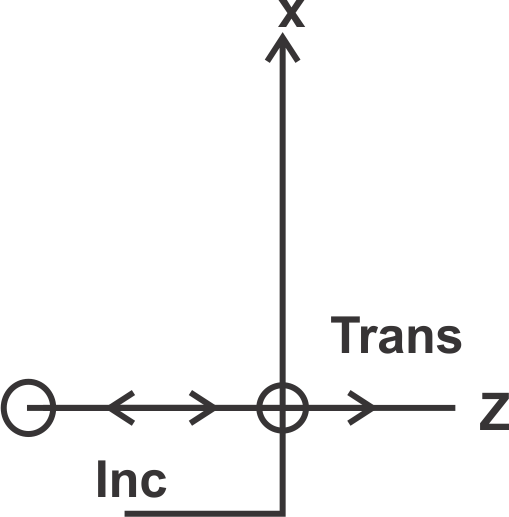
\includegraphics[scale=0.8]{./graphics/16}
\caption{}
\label{fig:16}
\end{figure}

At the condition $\theta_{i}$ = $\theta_{t}$ = 0 from equation 2.4 and 2.5 we have
\begin{equation}
\Gamma_{\perp} = \frac{\eta_{2} - \eta_{1}}{\eta_{2} + \eta_{1}}
\end{equation}
\begin{equation}
\tau_{\perp} = \frac{2 \eta_{2}}{\eta_{2} + \eta_{1}}
\end{equation}
We are not bothered about the variation of the field perpendicular to the transmission line. In this normal incidence case, perpendicular to the direction in which the wave is travelling, there is no field variation. At the interface looking rightward beyond the boundary, we see an infinite medium ahead of intrinsic impedance $\eta_{2}$. looking from the boundary to the right, we see another infinite medium with intrinsic impedance $\eta_{1}$. Hence it is like having two transmission lines having two characteristics impedance  $\eta_{2}$ and  $eta_{1}$.when the wave is incident from the left, it is like having a transmission  line with characteristics impedance  $\eta_{1}$ terminated in  $\eta_{2}$
\begin{figure}[h]
\centering

\includegraphics[width=.7\linewidth]{./graphics/17}
\caption{}
\label{fig:17}
\end{figure}

We get $\Gamma_{\perp} = \frac{\eta_{2} - \eta_{1}}{\eta_{2} + \eta_{1}}$ the reflection coefficent of a line with characteristics impedance  $\eta_{1}$ and terminated at  $\eta_{2}$.

So the case of normal incidence which is a special case for any oblique incidence at a dielectric interface is equivalent to the transmission line. So when we are dealing with a transmission line we are handling one of the special cases of reflections at the dielectric interface. When a transmission line is terminated in  $\eta_{21}$, the was getting lost in  $\eta_{2}$, now dating we have a dielectric interface,  either we say that the power is in  $\eta_{2}$ or the power is not lost at that location but going to the second medium. So the power lost at the dielectric boundary is the same as the power lost into  $\eta$ as the terminating impedance of the transmission line. 

For this normal incidence case with $\theta_{i}$ = $\theta_{t}$ = 0, for parallel polarization
\begin{dmath*}
\Gamma_{\perp} = \frac{\eta_{2} cos\theta_{i} - \eta_{1} cos\theta_{i}}{\eta_{2} cos\theta_{i} + \eta_{1} cos\theta_{t}}
= \frac{\eta_{2} - \eta_{1}}{\eta_{2} + \eta_{1}}
\end{dmath*}
while
\begin{dmath*}
\Gamma_{\parallel} = \frac{2 cos\theta_{i} \eta_{2}}{\eta_{2} cos\theta_{t} + \eta_{1} cos\theta_{i}} 
= \frac{\eta_{2} -\eta_{1}}{\eta_{2} +\eta_{1}}
\end{dmath*}
hence $\Gamma_{\perp}$ is opposite of $\Gamma_{\parallel}$

$\Gamma_{\perp}$ and $\Gamma_{\parallel}$ having opposite sign is due to the fact that for  $\Gamma_{\parallel}$,$E_{i}$ and $E_{r}$ had same direction. However, for  $\Gamma_{\parallel}$,$E_{i}$ and $E_{r}$ had opposite directions in the tangential component of the electric field that was used to solve for boundary condition. So the reflection coefficient in the case of normal incidence is written as $\Gamma = \frac{\eta_{1} - \eta_{2}}{\eta_{2} + \eta_{1}}$  with the assumption that electric field is in the same direction. If $\eta_{1}>\eta_{2}$ you have a phase reversal. If $\eta_{2}>\eta_{1}$ there is no phase reversal. 

So irrespective of the medium parameter and angle of incidence, the reflection and transmission coefficient are all real quantities. this may be direction reversal for the electric and magnetic fields,  but there is no arbitrary phase change either at the transmitted or reflected wave  .this case is a rather simple reflection and refraction case. 